\subsection{x86}

\subsubsection{\NonOptimizing MSVC}

\RU{Имеем в итоге}\EN{We got} (MSVC 2010):

\lstinputlisting[caption=MSVC 2010]{patterns/14_bitfields/2_set_reset/set_reset_msvc.asm}

\index{x86!\Instructions!OR}
\RU{Инструкция \OR здесь добавляет в переменную еще один бит, игнорируя остальные.}
\EN{\OR instruction adds one more bit to value while ignoring the rest ones.}

\index{x86!\Instructions!AND}
\RU{А \ANDIns сбрасывает некий бит. Можно также сказать, что \ANDIns здесь копирует все биты, кроме одного. 
Действительно, во втором операнде \ANDIns выставлены в единицу те биты, которые нужно сохранить, 
кроме одного, копировать который мы не хотим (и который $0$ в битовой маске).
Так проще понять и запомнить.}
\EN{\ANDIns resetting one bit. It can be said, \ANDIns just copies all bits except one.
Indeed, in the second \ANDIns operand only those bits are set, which are needed to be saved,
except one bit we would not like to copy (which is $0$ in bitmask).
It is easier way to memorize the logic.}

\myparagraph{\olly}

\RU{Попробуем этот пример в}\EN{Let's try this example in} \olly.
\RU{Сначала, посмотрим на двоичное представление используемых нами констант}
\EN{First, let's see binary form of constants we use}:

\TT{0x200} (0000000000000000000{\color{red}1}000000000) 
(\RU{т.е., 10-й бит (считая с первого)}\EN{i.e., 10th bit (counting from 1st)}).

\RU{Инвертированное}\EN{Inverted} \TT{0x200} \RU{это}\EN{is} \TT{0xFFFFFDFF} 
(1111111111111111111{\color{red}0}111111111).

\TT{0x4000} (00000000000000{\color{red}1}00000000000000) (\RU{т.е., 15-й бит}\EN{i.e., 15th bit}).

\RU{Входное значение это}\EN{Input value is}: \TT{0x12340678} (10010001101000000011001111000).
\RU{Видим, как оно загрузилось}\EN{We see how it's loaded}: \figref{fig:set_reset_olly1}.

\OR \RU{исполнилась}\EN{executed}: \figref{fig:set_reset_olly2}.
\RU{15-й бит выставлен}\EN{15th bit is set}: \TT{0x1234{\color{red}4}678} 
(10010001101000{\color{red}1}00011001111000).

\RU{Значение перезагружается снова (потому что использовался режим компилятора без оптимизации)}\EN{Value is 
reloaded again (because it's not optimizing compiler's mode)}: 
\figref{fig:set_reset_olly3}.

\ANDIns \RU{исполнилась}\EN{executed}: \figref{fig:set_reset_olly3}.
\RU{10-й бит очищен (или, иным языком, оставлены все биты кроме 10-го) и итоговое значение это}
\EN{10th bit is cleared (or, in other words, all bits are leaved instead of 10th) and final value now is} 
\TT{0x12344{\color{red}4}78} (1001000110100010001{\color{red}0}001111000).

\begin{figure}[H]
\centering
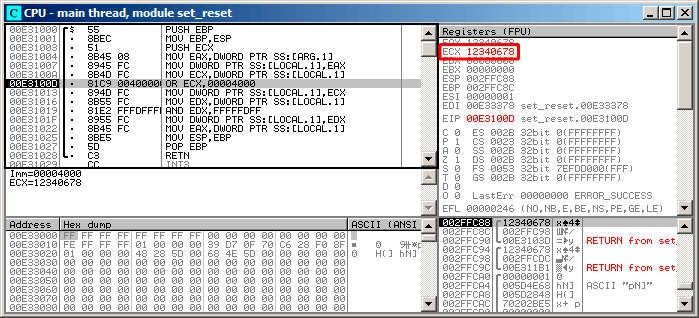
\includegraphics[scale=\FigScale]{patterns/14_bitfields/2_set_reset/olly1.png}
\caption{\olly: \EN{value is loaded into}\RU{значение загружено в} \ECX}
\label{fig:set_reset_olly1}
\end{figure}

\begin{figure}[H]
\centering
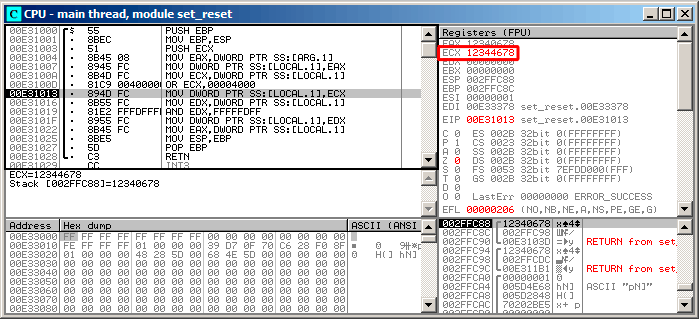
\includegraphics[scale=\FigScale]{patterns/14_bitfields/2_set_reset/olly2.png}
\caption{\olly: \OR \RU{сработал}\EN{executed}}
\label{fig:set_reset_olly2}
\end{figure}

\begin{figure}[H]
\centering
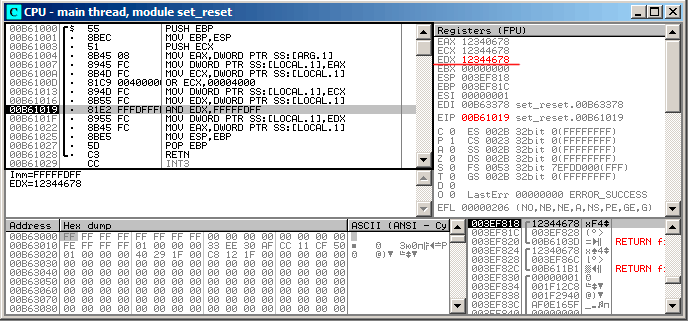
\includegraphics[scale=\FigScale]{patterns/14_bitfields/2_set_reset/olly3.png}
\caption{\olly: \EN{value was relaoded into}\RU{значение перезагрузилось в} \EDX}
\label{fig:set_reset_olly3}
\end{figure}

\begin{figure}[H]
\centering
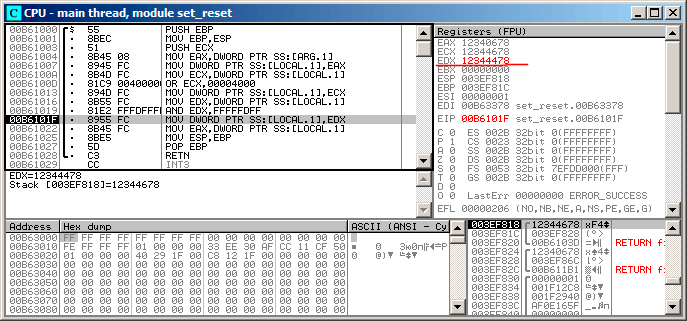
\includegraphics[scale=\FigScale]{patterns/14_bitfields/2_set_reset/olly4.png}
\caption{\olly: \ANDIns \RU{сработал}\EN{executed}}
\label{fig:set_reset_olly4}
\end{figure}

\subsubsection{\Optimizing MSVC}

\RU{Если скомпилировать в MSVC с оптимизацией (\Ox), то код будет еще короче:}
\EN{If we compile it in MSVC with optimization turned on (\Ox), the code will be even shorter:}

\lstinputlisting[caption=\Optimizing MSVC]{patterns/14_bitfields/2_set_reset/set_reset_msvc_Ox.asm}

\subsubsection{\NonOptimizing GCC}

\RU{Попробуем GCC 4.4.1 без оптимизации:}\EN{Let's try GCC 4.4.1 without optimization:}

\lstinputlisting[caption=\NonOptimizing GCC]{patterns/14_bitfields/2_set_reset/set_reset_gcc.asm}

\RU{Также избыточный код, хотя короче, чем у MSVC без оптимизации.}
\EN{There is a redundant code present,
however, it is shorter then MSVC version without optimization.}

\RU{Попробуем теперь GCC с оптимизацией}\EN{Now let's try GCC with optimization turned on} \Othree:

\subsubsection{\Optimizing GCC}

\lstinputlisting[caption=\Optimizing GCC]{patterns/14_bitfields/2_set_reset/set_reset_gcc_O3.asm}

\RU{Уже короче. Важно отметить что через регистр \AH, компилятор работает с частью регистра \EAX, 
эта его часть от 8-го до 15-го бита включительно.}
\EN{That's shorter.
It is worth noting the compiler works with the \EAX register part via the \AH 
register~---that is the \EAX register part from 8th to 15th bits inclusive.}

\RegTableOne{RAX}{EAX}{AX}{AH}{AL}

\index{x86!8086}
\index{x86!80386}
N.B. \RU{В 16-битном процессоре 8086 аккумулятор имел название \AX 
и состоял из двух 8-битных половин ~--- \AL (младшая часть) и \AH (старшая). 
В 80386 регистры были расширены до 32-бит, 
аккумулятор стал называться \EAX, но в целях совместимости, к его \IT{более старым} частям все еще можно 
обращаться как к \AX/\AH/\AL.}
\EN{16-bit CPU 8086 accumulator was named \AX and consisted of two 8-bit 
halves~---\AL (lower byte) and \AH (higher byte).
In 80386 almost all registers were extended to 32-bit, accumulator was named \EAX, 
but for the sake of compatibility,
its \IT{older parts} may be still accessed as \AX/\AH/\AL registers.}

\RU{Из-за того, что все x86 процессоры ~--- наследники 16-битного 8086, эти \IT{старые} 16-битные опкоды короче 
нежели более новые 32-битные. 
Поэтому, инструкция \TT{``or ah, 40h''} занимает только 3 байта. 
Было бы логичнее сгенерировать здесь \TT{``or eax, 04000h''}, но это уже 5 байт, или даже 6 
(если регистр в первом операнде не \EAX).}
\EN{Since all x86 CPUs are 16-bit 8086 CPU successors, these \IT{older} 16-bit opcodes are shorter 
than newer 32-bit opcodes.
That's why \TT{``or ah, 40h''} instruction occupying only 3 bytes.
It would be more logical way to emit here \TT{``or eax, 04000h''}
but that is 5 bytes, or even 6
(in case if register in first operand is not \EAX).}

\subsubsection{\Optimizing GCC \AndENRU regparm}

\RU{Если мы скомпилируем этот же пример не только с включенной оптимизацией \Othree, 
но еще и с опцией \TT{regparm=3}, о которой я писал немного выше, то получится еще короче:}
\EN{It would be even shorter if to turn on \Othree optimization flag and also set \TT{regparm=3}.}

\lstinputlisting[caption=\Optimizing GCC]{patterns/14_bitfields/2_set_reset/set_reset_gcc_O3_regparm3.asm}

\index{Inline code}
\RU{Действительно ~--- первый аргумент уже загружен в \EAX, и прямо здесь можно начинать с ним работать. 
Интересно, что и пролог функции (\TT{``push ebp / mov ebp,esp''}) и эпилог (\TT{``pop ebp''}) 
функции можно смело выкинуть
за ненадобностью, 
но возможно GCC еще не так хорош для подобных оптимизаций по размеру кода. 
Впрочем, в реальной жизни, подобные короткие функции лучше всего автоматически делать в виде 
\IT{inline-функций} (\ref{inline_code}).}
\EN{Indeed~---first argument is already loaded into \EAX, so it is possible to work with it in-place.
It is worth noting that both function prologue (\TT{``push ebp / mov ebp,esp''}) and epilogue (\TT{``pop ebp''})
can easily be omitted
here, but GCC probably is not good enough for such code size optimizations.
However, such short functions are better to be \IT{inlined functions} (\ref{inline_code}).}
